\subsection{Introduction}

The current kit comes with Ubuntu 12.04 installed on a MicroSD card. Using this 
operating system, we will learn to implement the following steps:
\begin{myitemize}
\item we will communicate with the devkit through UART
\item we will transfer of files between the host computer and the devkit through Ethernet
\item we will control the LEDs and the buzzer mounted on the devkit
\item we will read accelerometer data from the ADXL346 accelerometer mounted on the board
\item we will display the data using \textbf{bokeh}, which is a Python interactive visualization library
\item we will implement a webserver to visualize the accelerometer data, using as well \textbf{bokeh}
\end{myitemize}



\subsection{Let's get started!}

Now, we will move on with running an operating system on the System on Chip. For this, we will do the following steps:
\begin{myitemize}
\item you disconnected the JTAG cable used previously to programme the board
\item the mini SD Card is inserted in its socket (the filesystems are resided on a 4GB miniSD memory card where the board also boots from.)
\item find Jumper 1 and Jumper 2 (JP1 and JP2) and make sure they are in the following order:
\begin{minted}{c}
JP1 OFF 
JP2 ON
\end{minted}
\end{myitemize}



\subsection{Communication with the devkit through UART}

\begin{enumerate}
    \item Take the development kit and plug the microUSB into the USB\_UART socket (J6).  

    This connection enables serial communication between the host computer and the board, as well as power to the board.
    
    \item Open a terminal by pressing CTRL+ALT+T
    \item To communicate with the board, we will use \textbf{picocom} which is a very simple and straightforward terminal emulator. In your console, type:
        \begin{tcolorbox}
        \begin{minted}{c}
picocom -b 115200 /dev/ttyUSB0
        \end{minted}
        \end{tcolorbox}

    Now, what you will see (Figure \ref{fig:picocom}) is an emulator of the terminal of Ubuntu 12.04 running on the board.
    Type \textbf{reboot} and the system will re-start. After booting the board it gives you directly a bash shell as user root.


    \begin{figure}[h!]
    \centering
    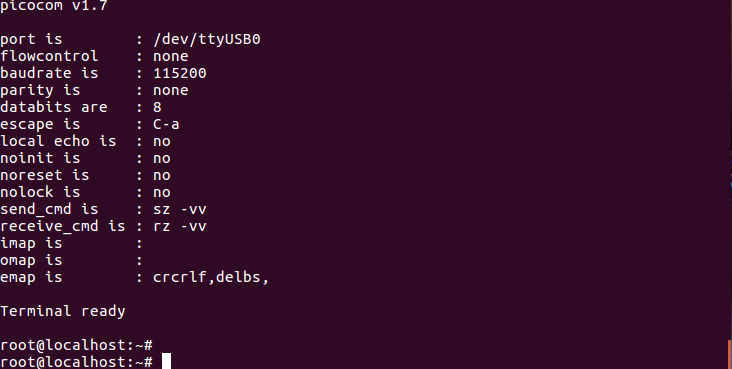
\includegraphics[width=0.7\textwidth]{img/picocom.png}
    \caption{Picocom Terminal Emulator}
    \label{fig:picocom}
\end{figure}


    \item Close the communication by pressing CTRL-A and then CTRL-X

    \item You shall see  \cref{appendix:graph} for other settings and installation process.
\end{enumerate}

{\color{red} \textbf{Optional:}} If you have a screen with an HDMI port, you can connect it to the board (Figure \ref{fig:hdmi}). You can also connect a mouse and a keyboard, but you will need a USB-OTG cable (miniUSB - to - standard USB).



\begin{figure}[h!]
    \centering
    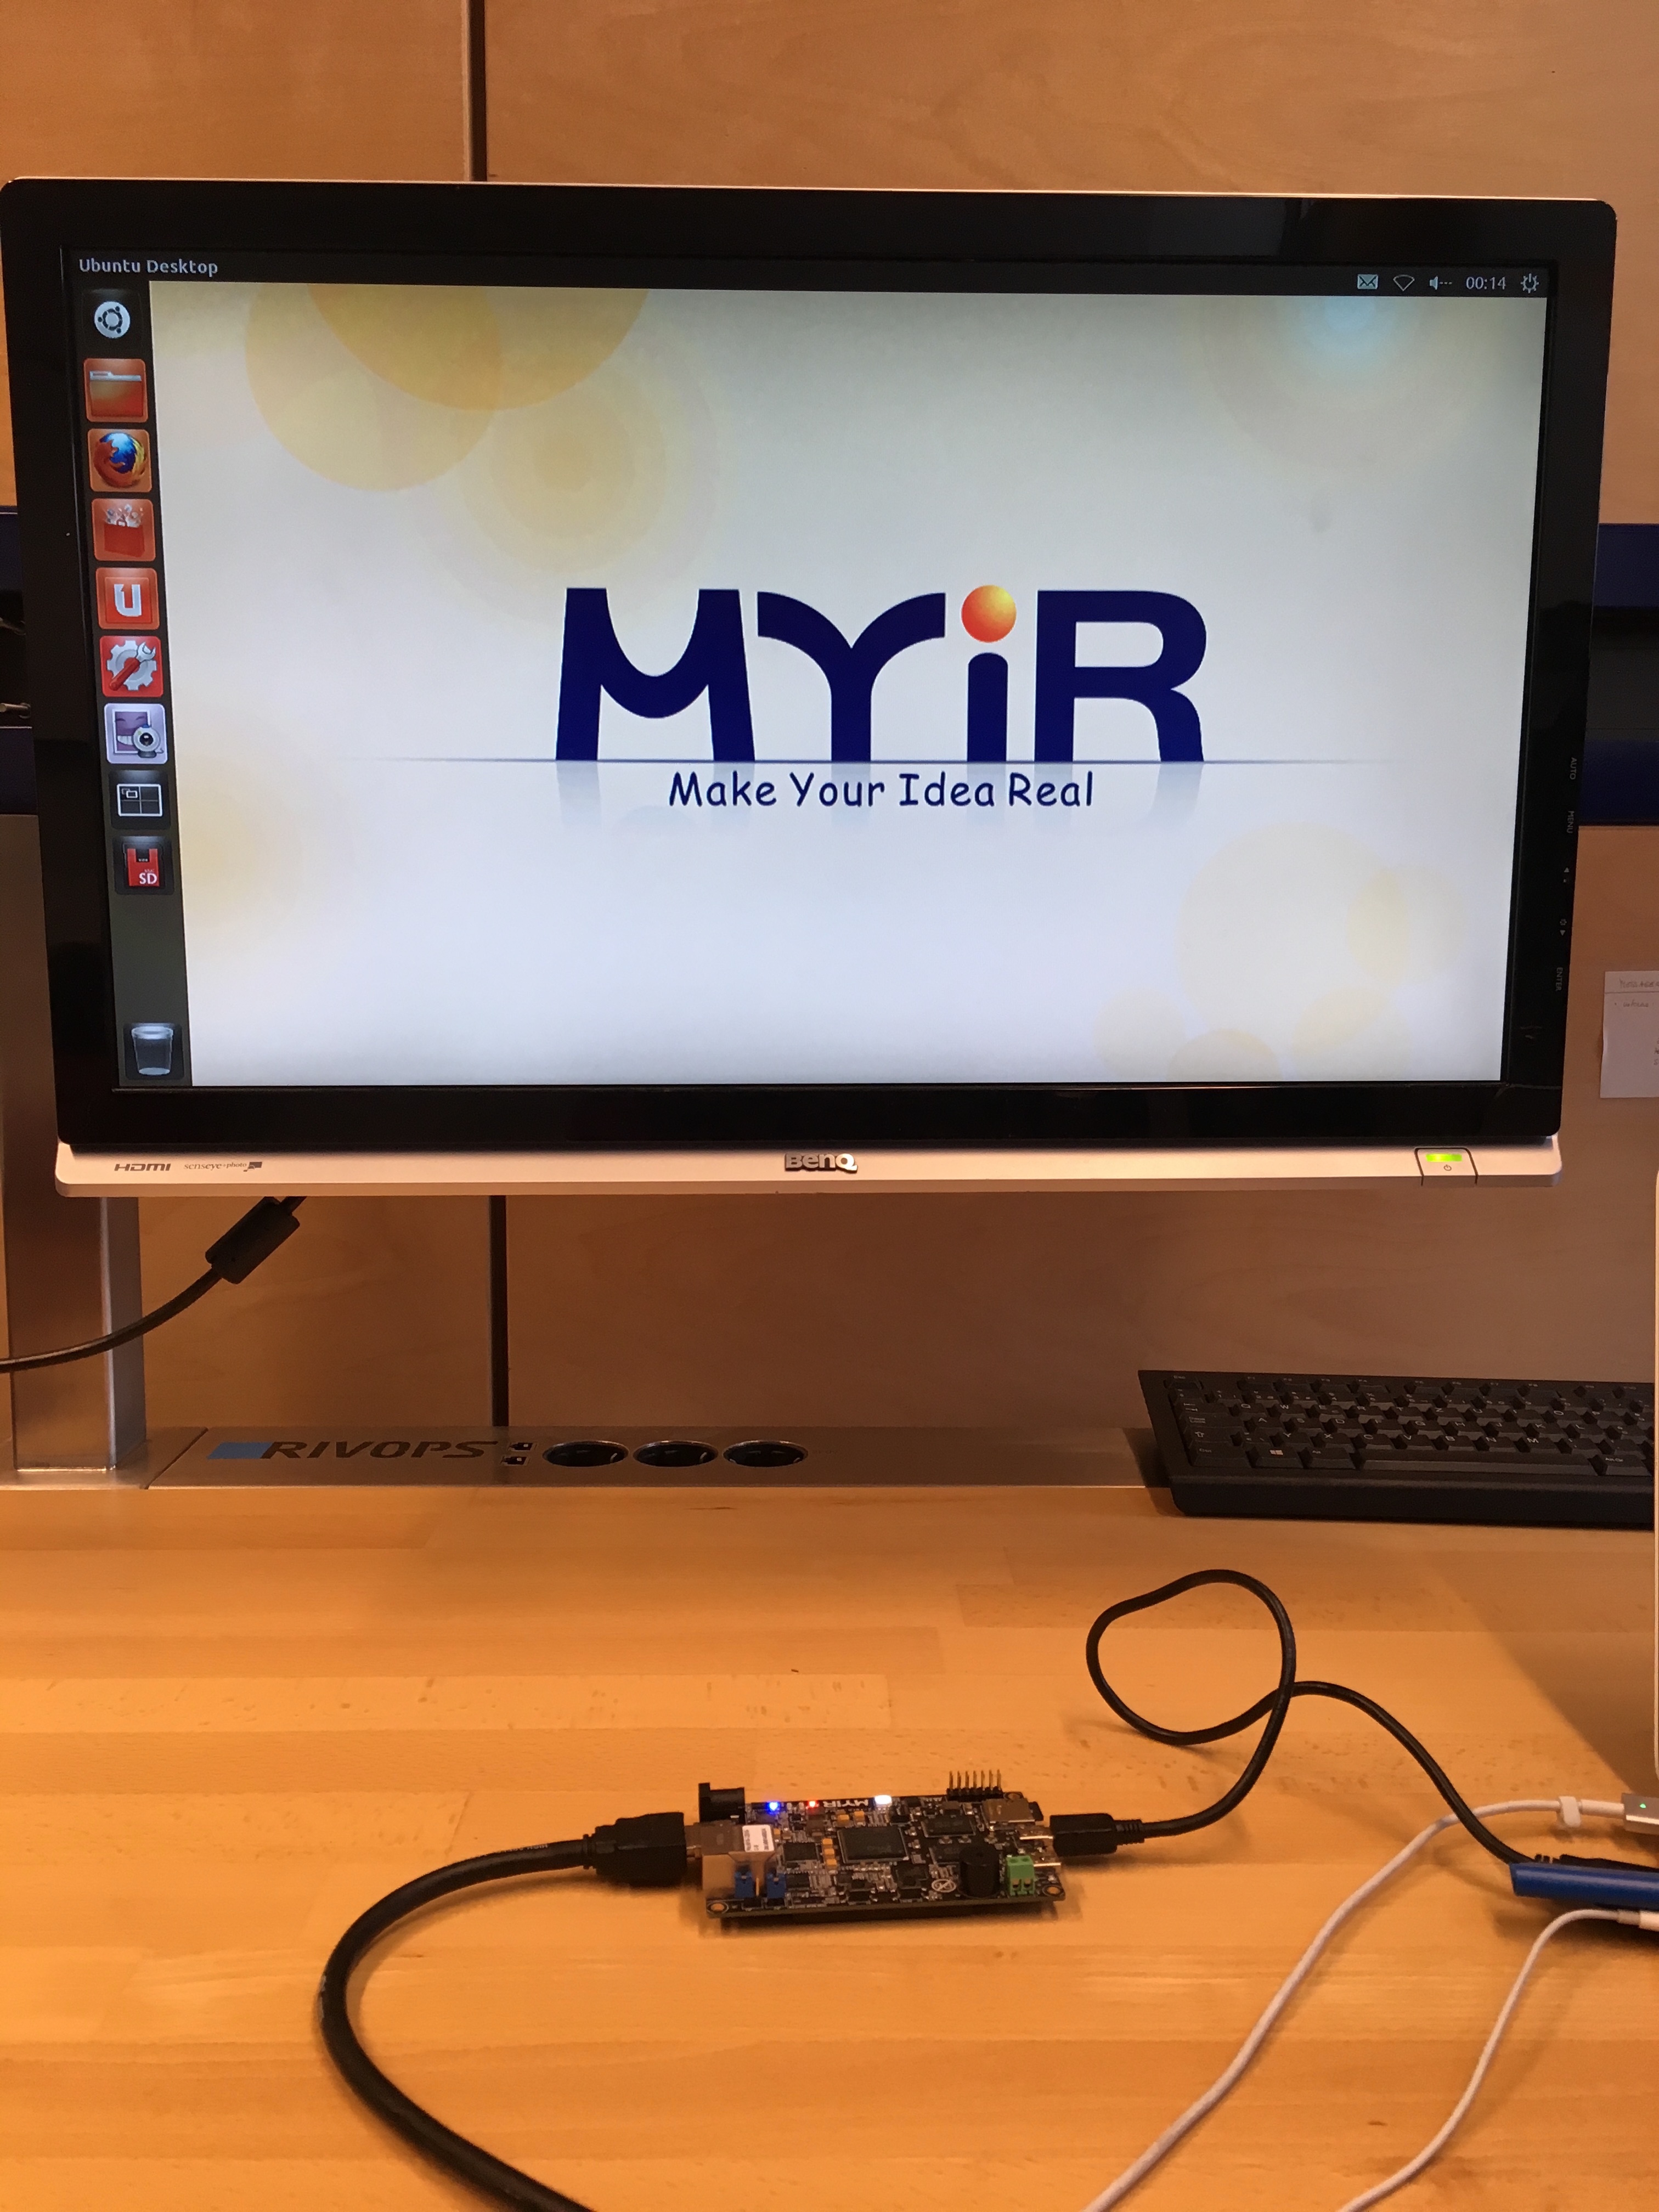
\includegraphics[width=0.6\textwidth]{img/hdmi.JPG}
    \caption{Screen connected to the board}
    \label{fig:hdmi}
\end{figure}


\clearpage
\subsection{Transfer of files between the host computer and the devkit}

In the current lab, we will develop source code on the host computer that needs to be transfered to the board.

There are three methods to transfer files:
\begin{myitemize}
\item Through UART serial protocol
\item Using SCP (Secure CoPy) - a simple transfer tool used to copy one or more files, often with known names, from host A (the computer) to host B (the board) or viceversa
\item Using SFTP (SSH File Transfer Protocol) - which is also a transfer tool used to copy files, but in addition it allows directory listings, remote directories and files removal, creation of files etc.
\end{myitemize}

To simplify life, we will use SCP. Never use UART unless you have a passion to encode/decode data or if other options are not available.

The SSH is already installed on the board. The settings can be seen in \cref{appendix:b}.

The following steps shall be performed: 
\begin{enumerate}
    \item Type in a new terminal the following command to connect to the board through SSH protocol.
    \begin{tcolorbox}
        \begin{minted}{c}
ssh root@192.168.2.2
        \end{minted}
    \end{tcolorbox}
    You will see basically the same emulator as before.

    \item Next, we will transfer a file to the board.

    On the Desktop, in folder \textit{Laboratory}, you will find a file entitled \textit{lab.py}. This part will contain the skeleton used to develop the next steps. Right now, we will just take this skeleton file and transfer it to the board.

    For this, \textbf{open a new terminal window} and type the next command in the box. The two points ":" at the end of the next command will place the file in the User folder.
    \begin{tcolorbox}
     \begin{minted}{c}
scp -r ~/Desktop/Laboratory/lab.py root@192.168.2.2:
    \end{minted}
    \end{tcolorbox}

\item Run lab.py

    \begin{tcolorbox}
     \begin{minted}{c}
python lab.py
    \end{minted}
    \end{tcolorbox}



\end{enumerate}













\subsubsection{How is LINUX OS interacting with both the accelerometer and the buzzer?}

The I/O subsystem is the part of the Linux kernel that manages the various devices such as keyboards and mouse, devices usually used by any users. On top of this, it comes the Industrial I/O subsystem (IIO) that are analog to digital or digital to analog convertors, for example \textbf{the accelerometer, gyroscopes, proximity sensors} with the aim to extend the I/O subsystem. A typical device falling into the IIO category would be connected via SPI or I2C.






\subsubsection{How is LINUX OS interacting with the LEDs?}




When previously steps are done, you will see the RGB LED blinking on the board. It is very
important to make these configurations before moving on to the next section of the lab.


The SD card contains the image of Ubuntu 12.04 and will boot it on the board at every restart.

\subsubsection{Screen}

\subsubsection{File transfer between host computer and the board}

% Connect a screen to see that it works

% Open a terminal and communicate 

% Send a file through SSH

\subsection{Interact with the RGB LED and the Buzzer}




\subsection{Webserver}
Now, we will learn how to display the accelerometer values on an webserver running
on the host computer.



 %Each device provides one or more /dev/input/eventN nodes that a process can interact with. For example  reading events from the device.


 %The events themselves are in the form of struct input_event, defined in linux/input.h and consist of a event type (relative, absolute, key, ...) and an event code specific to the type (x axis, left button, etc.).

 %Any event coming from the physical hardware goes into the kernel's input subsystem and is converted to an evdev event that is then available on the event node.
